\documentclass[preprint,12pt]{elsarticle}

\biboptions{numbers,sort&compress}
\usepackage{amsmath,amssymb}
\usepackage{array,booktabs}
\usepackage{microtype}
\usepackage{subcaption}
\usepackage{tabularx}
\usepackage{xspace}
\usepackage{graphicx}
\usepackage{url}
\usepackage{hyperref}
\hypersetup{hidelinks}
\pdfstringdefDisableCommands{%
  \def\corref#1{}%
  \def\cortext[#1]#2{}%
  \def\cormark[#1]{}%
  \def\ead#1{}%
  \def\address[#1]#2{}%
}
\emergencystretch=2em

\journal{Knowledge-Based Systems}
\graphicspath{{figures/}}
\newcommand{\method}{VulTriage\xspace}
\newcommand{\av}{\alpha_{\mathrm{v}}}
\newcommand{\as}{\alpha_{\mathrm{s}}}

\begin{document}
\begin{frontmatter}

\title{VulTriage: Proof-Carrying Detector--Shift Knowledge Contracts for Selective Vulnerability Triage}

\author[inst1]{Yanbo Bian\corref{cor1}}
\ead{24722081@bjtu.edu.cn}
\author[inst2]{Zhihai Wang}
\ead{zhhwang@bjtu.edu.cn}
\cortext[cor1]{Corresponding author: Yanbo Bian.}
\address[inst1]{Computer Science and Technology Program, Weihai International College, Beijing Jiaotong University, Weihai 264401, China}
\address[inst2]{School of Computer Science and Technology, Beijing Jiaotong University, Beijing 100044, China}

\begin{abstract}
\textbf{Problem:} Cross-project vulnerability detectors produce scores, but deployment requires a defensible answer to a different question: when is an automatic label permitted under asymmetric security costs? \textbf{Approach:} We present \method, which formulates selective automation as a proof-carrying detector--shift knowledge contract. Each contract binds a detector and source--target shift to a qualification registry, evaluates budget, evidence, gate, and singleton predicates in three-valued logic, and attaches a machine-verifiable certificate to every automatic action. False, unknown, mismatched, or unregistered evidence fails closed to review. \textbf{Methods:} A frozen, prediction-sealed study uses PrimeVul for retrospective controller development and 24 DiverseVul projects for evaluation with hashing-SGD and a frozen CodeBERT encoder. An exploratory contract extension uses a deterministic 12/12 registration--confirmation split and 10,000 deterministic split perturbations without removing any frozen result. \textbf{Results:} Hashing-SGD is registered with qualification score $Q=0.757$ and confirms at $Q=0.917$; on the confirmation half the contract sends five of six severe projects to review and releases all six non-severe projects as eligible for singleton automation. Both halves exceed $Q=0.70$ in 84.94\% of 10,000 splits. The registry withholds CodeBERT authority ($Q=0.150$), so all of its confirmation projects remain review-only. Independently, project-aware weighting improves hashing risk alignment on all 24 projects at the primary operating point and on 202 of 216 project--budget cells, with the direction preserved under calibration-size and near-duplicate sensitivity analyses. \textbf{Implications:} \method turns uncertainty evidence into inspectable automation authority and makes unsupported detector transfer mechanically non-authorizing.
\end{abstract}

\begin{keyword}
  proof-carrying knowledge contract \sep vulnerability detection \sep conformal prediction \sep selective classification \sep dataset shift
\end{keyword}
\end{frontmatter}

\section{Introduction}

A vulnerability detector deployed on an unseen software project must answer two different questions. The predictive question is which functions look vulnerable. The decisional question is whether the detector currently possesses enough evidence and authority to release an automatic label. This distinction is consequential: a missed vulnerable function and an unnecessary alert consume different resources, project shift can invalidate calibration evidence, and a confidence score contains no explicit statement about which detector, shift, budget, or evidence state it authorizes. A knowledge-based decision-support system therefore needs more than uncertainty estimation. It needs an executable permission model for automation.

Public vulnerability benchmarks have made the first question more realistic. PrimeVul reports the effects of duplicate functions, label quality, imbalance, and evaluation design on code-language-model results \cite{ding2025primevul}, while DiverseVul broadens project and weakness coverage for deep vulnerability detection \cite{chen2023diversevul}. Cross-project methods address representation and distribution mismatch with transfer learning, domain adaptation, graph representations, and zero-shot mechanisms \cite{lin2018transfer,liu2022cdvuld,zhang2023cpvd,nguyen2024dam2p,cai2024csvdtf,haque2026zsvuld}. These methods improve or adapt a detector, but a deployment still needs an explicit policy for returning a label, deferring to review, and reporting the cost of that refusal.

Calibration and selective prediction provide important ingredients. CodeBERT is a standard pretrained representation for source code \cite{feng2020codebert}, and LineVul and data-flow-aware models show how detector architecture can be improved \cite{fu2022linevul,steenhoek2024deepdfa}. Temperature scaling is a canonical calibration baseline \cite{guo2017calibration}, while selective prediction formalizes the risk--coverage trade-off \cite{geifman2019selectivenet}. Code-model calibration can degrade under shift \cite{zhou2024calibration}, and Prom provides deployment-time conformal assessment for code-analysis tasks \cite{wang2025prom}. Recent work also frames code prediction as an answer-or-defer decision \cite{rathnasuriya2026defer}; a KBS study connects uncertainty estimation under dataset shift to malware-classification decisions \cite{yumlembam2026kbs}. Most closely, AEGIS separates learned vulnerability perception from a symbolic Block/Warn/Pass policy guard in CI/CD \cite{abdallah2026aegis}. This establishes policy-governed vulnerability management, but leaves a sharper deployment question: how can automation authority be bound to a particular detector--shift identity, withheld before item-level execution, and carried by a machine-verifiable decision object?

We address this gap with \method, a post-hoc decision layer that wraps a fitted detector with a proof-carrying detector--shift knowledge contract. The detector and source--target shift form a versioned identity. A qualification registry decides whether evidence learned for that identity may authorize automation. At runtime, four policy predicates---valid asymmetric budgets, complete evidence, qualified detector--shift support, and singleton eligibility---are evaluated in three-valued logic. Only a conjunction of true predicates creates an automation entitlement; every other state produces review. The emitted decision certificate records the contract identity, risk budget, rule truth values, action, and evidence digest and is independently verifiable. Thus, \method separates three concerns that score-based pipelines conflate: evidence generation, authority qualification, and action execution.

The empirical layer combines class-conditional conformal sets with estimated source-to-target relevance weights and a frozen, label-free severe-risk gate. The project, rather than an individual function or random row, is the unit of deployment and inference. We evaluate both the underlying risk alignment and the higher-level authority contract. The latter uses a fixed hash-defined registration--confirmation partition and deterministic split perturbations to test whether qualification is a stable property of a detector--shift identity rather than an artifact of one convenient partition.

The study asks:

\begin{itemize}
  \item \textbf{RQ1:} Can an executable knowledge contract transform uncertainty evidence into mechanically verifiable automation authority with fail-closed semantics?
  \item \textbf{RQ2:} Can detector--shift qualification distinguish supported automation from unsupported transfer, and is that decision stable across project partitions?
  \item \textbf{RQ3:} How strongly does project-aware weighting improve class-asymmetric risk alignment, and does the gain persist under calibration-size and duplicate-control sensitivity analyses?
\end{itemize}

The contributions are fourfold:

\begin{enumerate}
  \item an executable proof-carrying knowledge contract that binds detector--shift identity, three-valued evidence rules, fail-closed entitlement logic, and independently verifiable decision certificates;
  \item a detector-specific qualification registry based on a composite discrimination-and-triage score, together with fixed hash-defined registration--confirmation evaluation and 10,000 deterministic partition perturbations;
  \item a frozen, prediction-sealed external evaluation showing that project-aware weighting improves hashing-SGD risk alignment on all 24 projects at the primary operating point and on 202 of 216 project--budget cells, with quantified automation cost and sensitivity evidence; and
  \item a positive governance result: the same qualification firewall that registers hashing-SGD blocks unsupported CodeBERT transfer by construction, while released code, tables, certificates, figure source data, and manifests make the evidence chain inspectable.
\end{enumerate}

\section{Related work}

\subsection{Cross-project vulnerability detection and decision support}

Representation transfer for vulnerable-function discovery predates current code-language models \cite{lin2018transfer}. CD-VulD combines deep domain adaptation with cross-domain vulnerability discovery \cite{liu2022cdvuld}. CPVD uses graph attention and domain adaptation \cite{zhang2023cpvd}, DAM2P introduces a max-margin domain-adaptation objective for imbalanced data \cite{nguyen2024dam2p}, and CSVD-TF uses TrAdaBoost to fuse expert and semantic metrics \cite{cai2024csvdtf}. ZSVulD studies a zero-shot setting with pretrained representations and collaborative classifiers \cite{haque2026zsvuld}. These systems change the detector or its training objective. \method is complementary: it takes a fitted detector and exposes a decision layer that can refuse unsupported automation.

Software-engineering studies also emphasize the operational side of vulnerability prediction. A systematic mapping study organizes the evidence base and its evaluation practices \cite{kalouptsoglou2023mapping}; comparative work shows that vulnerability predictors can behave differently across models and projects \cite{theisen2020better}; and a practical framework separates prediction, categorization, and localization rather than treating a single classifier score as the complete workflow \cite{liu2024practical}. These studies motivate a project-level decision-support layer that makes refusal cost and class-asymmetric risk explicit. \method does not claim to replace those detectors or to provide a new vulnerability representation.

\subsection{Knowledge-based uncertainty and security decision support}

Recent contributions in \textit{Knowledge-Based Systems} illustrate the target perspective. Yumlembam et al. connect uncertainty estimation with malware-classification decisions under dataset shift \cite{yumlembam2026kbs}, while Wijekoon and Wiratunga evaluate user-facing counterfactual support for code vulnerability detection and correction \cite{wijekoon2023discern}. Other KBS studies focus on improving the detector or the vulnerability score itself, including function fingerprints and code differences \cite{zhao2023vuldeff} and lightweight vulnerability-score prediction \cite{mirtaheri2025vulscore}. Our contribution is complementary: the learned detector remains fixed, and the knowledge component is an explicit, inspectable policy that maps uncertainty evidence to automatic or review actions. We therefore evaluate whether this policy transfers across detector--shift pairs rather than presenting it as a new ontology, expert knowledge graph, or detector state of the art.

The closest conceptual neighbor is AEGIS, which combines graph-based risk estimation, stochastic epistemic uncertainty, and symbolic action constraints for auditable CI/CD decisions \cite{abdallah2026aegis}. \method advances this policy-governance direction through a different knowledge mechanism: a versioned detector--shift identity first acquires or is denied authority in a qualification registry; three-valued predicates prevent missing evidence from becoming permission; and each automatic action carries a certificate that a verifier checks by re-executing the complete contract. Registration--confirmation separation and partition perturbations then evaluate whether that authority is stable, not merely whether a fixed policy can be replayed. These mechanisms make detector transfer an executable access-control question rather than a threshold-reuse convention.

Proof-carrying code established the architectural pattern in which a producer supplies evidence that a consumer can validate against a previously defined policy \cite{necula1997pcc}. \method transfers that pattern to decision governance rather than program safety: its certificate attests that a serialized triage contract was executed consistently for a detector--shift identity. It does not prove that source code is safe, that the detector is correct, or that a conformal risk guarantee holds under arbitrary shift.

Modern code detectors provide important external-validity baselines. CodeBERT supplies a pretrained code representation \cite{feng2020codebert}, LineVul adapts transformers to line-level vulnerability prediction \cite{fu2022linevul}, and DeepDFA injects data-flow structure for efficient detection \cite{steenhoek2024deepdfa}. Our CodeBERT track is deliberately a frozen encoder plus a source-train-only standardized logistic head, not a claim of fine-tuned state of the art. The contrast with hashing-SGD therefore tests whether support-aware weighting behaves consistently across a low-cost lexical detector and a semantic representation. These studies primarily optimize or compare detectors; \method addresses the complementary software-engineering task of deciding when detector output is ready for automatic release and when it must remain in a review queue.

\subsection{Selective automation and conformal risk}

Temperature scaling changes probability calibration but not the binary ranking \cite{guo2017calibration}. Selective prediction makes retained coverage an explicit companion to risk \cite{geifman2019selectivenet}, and code-model studies show that calibration remedies can behave differently under project or temporal shift \cite{zhou2024calibration,li2021shift}. Prom uses local conformal experts, including LAC, TopK, APS, and RAPS, to identify deployment-time errors in code analysis \cite{wang2025prom}. We use a pre-specified binary, deterministic PROM-derived adapter as a strong comparison, while distinguishing it from the official implementation. The answer-or-defer perspective for code prediction is also established \cite{rathnasuriya2026defer}; our focus is the security-specific separation of vulnerable and safe budgets and the validity of an unlabeled support signal.

Weighted conformal prediction can recover target marginal coverage under covariate shift when the likelihood ratio is known and conditional labels are invariant \cite{tibshirani2019weightedcp}. Conformal risk control generalizes the controlled loss \cite{angelopoulos2024crc}, and nonexchangeable or high-probability variants make the shift assumptions explicit \cite{farinhas2024necrc,almeida2025hpcrc}. Our density ratios are learned from a finite domain classifier and project shift may include concept shift. We therefore report empirical violation, support diagnostics, and refusal cost rather than claiming a distribution-free deployment guarantee.

\section{Proof-carrying detector--shift knowledge contracts}

\subsection{Contract identity and qualification registry}

We separate evidence generation from the authority to act on that evidence. A contract identity is
\begin{equation}
 \iota=(d,\mathcal S,\mathcal T,v),
 \label{eq:identity}
\end{equation}
where $d$ is the fitted detector family, $\mathcal S$ and $\mathcal T$ are the source and target domains, and $v$ is the policy version. A cryptographic digest of these fields supplies the contract identifier. Consequently, a qualification learned for hashing-SGD under PrimeVul$\rightarrow$DiverseVul is not addressable as a CodeBERT qualification, even when both detectors process the same projects.

The registry $\mathcal R(\iota)\in\{0,1\}$ stores whether identity $\iota$ is eligible to request runtime automation. Qualification combines ranking and threshold behavior. Let $A$ be the severe-violation AUROC of the label-free gate, $r_{\mathrm{sev}}$ the fraction of severe projects routed to review, and $p_{\mathrm{non}}$ the fraction of non-severe projects passed. We define
\begin{equation}
 B=\frac{r_{\mathrm{sev}}+p_{\mathrm{non}}}{2},
 \qquad
 Q=\min(A,B),
 \qquad
 \mathcal R(\iota)=\mathbf 1\{Q\geq\eta\},
 \label{eq:qualification}
\end{equation}
with $\eta=0.70$. The minimum prevents strong ranking from compensating for a poor deployed threshold, or vice versa. Qualification is a detector--shift governance decision evaluated after labels are available; runtime contract execution still consumes only the registered identity, unlabeled evidence, gate output, and prediction set.

\subsection{Three-valued evidence logic and certificates}

For a target project and requested budget $\boldsymbol{\alpha}=(\av,\as)$, four predicates carry values in $\mathbb V=\{\mathsf T,\mathsf F,\mathsf U\}$:
\begin{align}
 K_1 &: \text{the two risk budgets are finite and valid},\nonumber\\
 K_2 &: \text{the required support evidence is complete},\nonumber\\
 K_3 &: \text{the detector--shift identity is registered and the gate passes},\nonumber\\
 K_4 &: \text{the prediction set is a valid singleton}. \label{eq:rules}
\end{align}
Conjunction follows strong Kleene logic: any false operand makes the entitlement false; otherwise any unknown operand makes it unknown; only all-true evidence yields true. The automation entitlement is
\begin{equation}
 E(\iota,x)=K_1\wedge K_2\wedge K_3\wedge K_4.
 \label{eq:entitlement}
\end{equation}
The fifth knowledge rule is operational: $K_5$ maps every false or unknown entitlement to review and requires a proof object for each automatic action. For evidence payload $e$, the certificate is
\begin{equation}
 C=\bigl(\mathrm{id}(\iota),\boldsymbol{\alpha},\Gamma(x),
          K_1{:}K_4,E,\pi,H(e)\bigr),
 \label{eq:certificate}
\end{equation}
where $H(e)$ is a SHA-256 evidence digest and $\pi$ is the action. Given the expected identity and evidence record, a verifier re-executes the contract and requires an exact certificate match. Identity, payload, budget, prediction-set, entitlement, and action substitutions are therefore rejected.

\begin{table*}[t]
\centering
\caption{Executable knowledge rules in the detector--shift contract. K1--K4 construct an entitlement in three-valued logic; K5 makes the decision fail closed and requires a verifiable certificate.}
\label{tab:knowledge_rules}
\small
\renewcommand{\arraystretch}{1.12}
\begin{tabularx}{\textwidth}{@{}>{\raggedright\arraybackslash}p{0.06\textwidth}>{\raggedright\arraybackslash}p{0.19\textwidth}>{\raggedright\arraybackslash}X>{\raggedright\arraybackslash}p{0.25\textwidth}@{}}
\toprule
Rule & Knowledge item & Runtime interpretation & Audit record \\
\midrule
K1 & Budget binding & Validate and bind $\alpha_{\mathrm v}$ and $\alpha_{\mathrm s}$ to the decision. & Budget pair and class-wise outcomes. \\
K2 & Evidence completeness & Record ESS, infinity mass, domain AUROC, and clipping fractions; missing evidence is unknown. & Evidence payload and digest. \\
K3 & Qualified identity & Require detector--shift identity registration and a passing severe-risk gate. & Contract ID, registry version, gate score. \\
K4 & Singleton eligibility & Require $\Gamma(x)\in\{\{0\},\{1\}\}$ before automatic action. & Prediction set and candidate action. \\
K5 & Proof-carrying fail closure & Route false, unknown, mismatched, or unregistered states to review; certify automatic actions. & Truth values, entitlement, action, SHA-256 digest. \\
\bottomrule
\end{tabularx}
\end{table*}

Given a prediction set $\Gamma(x)$, the action policy is
\begin{equation}
\pi_{\mathcal K}(x,z,\Gamma,\iota)=
\begin{cases}
\textsf{auto-vulnerable}, & E(\iota,x)=\mathsf T\ \text{and}\ \Gamma(x)=\{1\},\\
\textsf{auto-safe}, & E(\iota,x)=\mathsf T\ \text{and}\ \Gamma(x)=\{0\},\\
\textsf{review}, & \text{otherwise}.
\end{cases}
\label{eq:action_policy}
\end{equation}

\paragraph{Property 1 (automatic-action soundness).}
Relative to the serialized contract, a verified automatic certificate implies $K_j=\mathsf T$ for every $j\in\{1,2,3,4\}$ and an action consistent with the recorded singleton. This follows directly from Eqs.~\eqref{eq:entitlement}--\eqref{eq:action_policy} and the verifier's action--singleton check.

\paragraph{Property 2 (fail-closed monotonicity under evidence loss).}
Replacing any true predicate with false or unknown cannot change a review action into an automatic action. Under strong Kleene conjunction, the entitlement can only remain true when every predicate remains true.

\paragraph{Property 3 (detector-transfer non-interference).}
Registration of identity $\iota$ cannot authorize $\iota'\neq\iota$. The contract identifier binds $d$, $\mathcal S$, $\mathcal T$, and $v$, and $K_3$ is false on an identity mismatch. These are semantic guarantees of the executable policy, distinct from claims about predictive accuracy or conformal coverage.

\begin{figure*}[t]
  \centering
  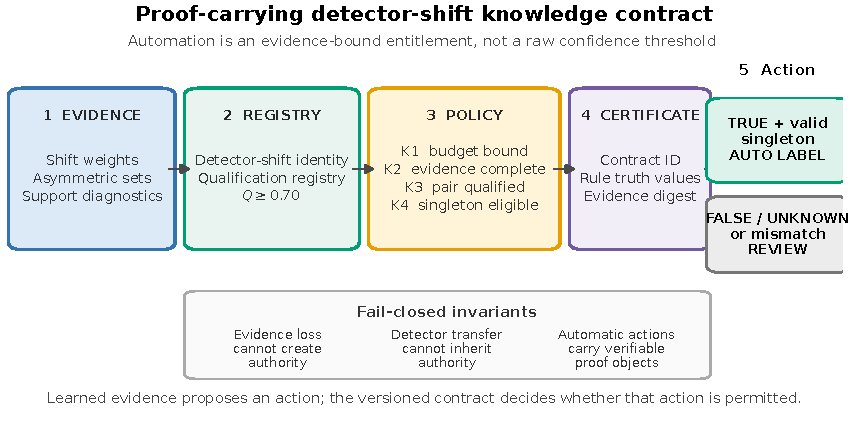
\includegraphics[width=0.97\textwidth]{fig1_workflow.pdf}
  \caption{\method treats automation as an evidence-bound entitlement. The evidence engine supplies shift weights, asymmetric sets, and support diagnostics; the registry binds qualification to a detector--shift identity; K1--K4 evaluate three-valued evidence; and K5 permits an automatic label only with a verifiable certificate. Evidence loss, identity mismatch, failed qualification, or a non-singleton prediction closes the action to review.}
  \label{fig:workflow}
\end{figure*}

\subsection{Uncertainty sets and three-way actions}

Let $Y\in\{0,1\}$ denote safe and vulnerable, respectively, and let a fitted detector output class probabilities $\widehat p_y(x)$. For calibration example $(x_i,y_i)$, the label-conditional nonconformity score is

\begin{equation}
 S_i=1-\widehat p_{y_i}(x_i).
\end{equation}

The output $\Gamma(x)\subseteq\{0,1\}$ has three operational interpretations. $\{0\}$ and $\{1\}$ are singleton automatic decisions; $\{0,1\}$ is a review decision. Empty sets, which can arise in comparison methods, are also routed to review and are recorded separately. For class $y$, the empirical miscoverage is

\begin{equation}
 R_y=\Pr\{y\notin\Gamma(X)\mid Y=y\}.
\end{equation}

The user supplies $\alpha_1=\av$ and $\alpha_0=\as$. Singleton coverage is $\Pr(|\Gamma(X)|=1)$ and review load is its complement.

\subsection{Asymmetric weighted sets}

For class $y$, let $\mathcal I_y$ be its calibration indices and let $w_i$ be estimated target relevance weights. For a target point with weight $w(x)$, the implemented threshold is

\begin{equation}
q_y(x)=\inf\left\{t:\sum_{i\in\mathcal I_y} w_i\mathbf 1(S_i\leq t)\geq(1-\alpha_y)\left(\sum_{i\in\mathcal I_y}w_i+w(x)\right)\right\}.
\label{eq:weighted}
\end{equation}

If the calibration mass cannot reach the right-hand side, $q_y(x)=\infty$. The set contains class $y$ when $1-\widehat p_y(x)\leq q_y(x)$. Unit weights recover unweighted Mondrian conformal prediction. The weighted construction is an empirical post-processing rule: its exact covariate-shift validity would require a correct likelihood ratio and invariant conditional labels \cite{tibshirani2019weightedcp}.

\subsection{Project-shift weights and support gate}

For each held-out project, a source--target domain classifier is trained with five deterministic cross-fitting folds. Equal source and target sampling makes the cross-fitted target odds

\begin{equation}
 \widehat w(x)=\frac{\widehat P(D=1\mid x)}{1-\widehat P(D=1\mid x)}
\end{equation}

an estimated relevance ratio. The primary weights are clipped to $[1/20,20]$; clips 10 and 50 are sensitivity variants. The same label-free weights are shared by detector-head seeds.

The frozen support gate is fitted only on 12 PrimeVul project-disjoint pseudo-targets using leave-one-project-out cross-fitting. Its features are log total and class-specific Kish effective sample sizes (ESS), maximum and 99th-percentile test-point infinity mass, domain-classifier AUROC, and lower and upper clipping fractions. The gate predicts whether the raw weighted policy will have severe relative violation, defined as

\begin{equation}
 \max\left(\frac{\max(0,R_1-\av)}{\av},\frac{\max(0,R_0-\as)}{\as}\right)>0.5.
\end{equation}

The frozen gate $G(z)$ passes only when its fixed logistic score (interpreted as an estimated severe-violation probability, without post-hoc target calibration) is below $\tau_{\mathrm{sev}}=0.5$, the evidence vector is finite, and at least one singleton exists. Missing or nonfinite diagnostics fail closed. A failed gate replaces the entire target-project cell with review sets. This is a conservative knowledge rule, not evidence that the requested risks have been attained. The development fit contains 12 independent projects and nine correlated budget rows per project; the resulting 108-row AUROC is therefore descriptive rather than an independent-sample estimate.

\section{Empirical evaluation of the decision-support system}

\subsection{Study protocol and analysis unit}

The study follows a frozen, prediction-sealed external-evaluation protocol organized around the software-project unit of deployment. PrimeVul is used for retrospective development and gate fitting, whereas DiverseVul supplies the external project groups. Target labels are withheld until detector predictions and support diagnostics are sealed. The learned weighting component and the proof-carrying contract are evaluated as separate decision-support components. The primary comparison is estimated weighting versus unweighted Mondrian sets at $(\av,\as)=(0.10,0.20)$ within each detector; the remaining budget cells, calibration fractions, duplicate audit, and efficiency measurements are sensitivity or descriptive analyses. Five seeds are technical replicates nested within a project, so inference is performed on the 24 external projects rather than on individual functions or seed--project rows.

\subsection{Datasets and project splits}

The development domain is the original public PrimeVul release \cite{ding2025primevul}. After deterministic canonicalization and exact deduplication, the source package contains 226,582 functions from 235,768 valid rows; 9,186 same-label duplicates are removed and no conflicting label keys are retained. For each external target, source rows are partitioned by salted commit-hash buckets into 70\% detector training, 10\% model validation, and 20\% calibration. Project aliases are frozen before model output.

The external evaluation domain is the official public DiverseVul release \cite{chen2023diversevul}. We select 24 eligible project groups without inspecting model outcomes, require at least 200 total, 20 vulnerable, and 20 safe functions, and then exact-deduplicate across datasets. Eligibility uses target label counts only to exclude one-class or very small projects; it is a cohort-design criterion rather than an outcome-based selection, but it limits prevalence generalization. The resulting target cohort contains 79,355 functions. Labels remain in a separate vault until both detector prediction seals are verified. The primary cohort is unchanged by the near-duplicate sensitivity analysis.

\begin{table*}[t]
\centering
\caption{DiverseVul external project groups. Target rows are exact-deduplicated functions; vulnerability prevalence is reported only descriptively after label release.}
\label{tab:projects}
\small
\setlength{\tabcolsep}{3pt}
\resizebox{\textwidth}{!}{%
\begin{tabular}{lrrr@{\qquad}lrrr}
\toprule
Project & Total & Vulnerable & Prev. (\%) & Project & Total & Vulnerable & Prev. (\%)\\
\midrule
linux & 32,930 & 3,032 & 9.21 & openssl & 4,352 & 565 & 12.98\\
tensorflow & 2,677 & 438 & 16.36 & php & 3,592 & 353 & 9.83\\
qemu & 2,634 & 338 & 12.83 & imagemagick & 783 & 300 & 38.31\\
qpdf & 1,786 & 272 & 15.23 & envoy & 5,252 & 254 & 4.84\\
tcpdump & 428 & 209 & 48.83 & jasper & 608 & 203 & 33.39\\
radare2 & 1,610 & 168 & 10.43 & postgres & 2,605 & 154 & 5.91\\
mysql-server & 3,838 & 142 & 3.70 & FreeRDP & 980 & 141 & 14.39\\
libxml2 & 2,060 & 136 & 6.60 & krb5 & 491 & 118 & 24.03\\
samba & 1,961 & 117 & 5.97 & vim & 3,056 & 116 & 3.80\\
net & 1,810 & 116 & 6.41 & ffmpeg & 983 & 115 & 11.70\\
mongo & 2,627 & 112 & 4.26 & ghostpdl & 1,132 & 109 & 9.63\\
libtpms & 490 & 109 & 22.24 & librsvg & 670 & 95 & 14.18\\
\bottomrule
\end{tabular}
}%
\end{table*}

\subsection{Detectors and comparison methods}

The lightweight detector hashes case-sensitive word unigrams and bigrams into $2^{18}$ dimensions, applies $\ell_2$ normalization, and fits a class-balanced averaged-SGD logistic head for three epochs. Regularization is selected by source-validation PR-AUC. Seeds 13, 37, 73, 101, and 137 are five independently fitted technical seeds per project.

The semantic track uses \texttt{microsoft/codebert-base} at immutable revision \texttt{3b0952feddeffad0063f274080e3c23d75e7eb39}. Final hidden states are attention-mask mean pooled after removing special tokens. A source-train-only StandardScaler feeds a class-weighted L2 liblinear logistic head; $C\in\{0.01,0.1,1,10\}$ is selected on source validation. CodeBERT is fitted once at seed 13 per project and the deterministic head is copied to the other four frozen seed addresses. This is a reproducibility address scheme, not five independent CodeBERT fits.

The evaluation records forced argmax, matched maximum-softmax and entropy, temperature-matched confidence, pooled and unweighted conformal sets, a binary PROM-derived adapter (LAC, TopK, APS, RAPS, and their union), estimated weighting with clips 10/20/50, ESS-only and infinity-mass-only gates, the full frozen gate, and matched full-gate derivatives. The PROM comparison is explicitly a deterministic binary adapter, not an official PROM reproduction \cite{wang2025prom}.

\subsection{Outcomes, sealing, and statistics}

We evaluate nine pre-specified budget pairs: $\av\in\{0.01,0.05,0.10\}$ and $\as\in\{0.05,0.10,0.20\}$. Primary outcomes are vulnerable and safe miscoverage, positive class-specific violation, maximum relative violation, singleton coverage, and review load. Detector performance includes PR-AUC, F1, Matthews correlation coefficient (MCC), Brier score, expected calibration error, area under the risk--coverage curve, and error-detection AUROC. The latter ranks forced 0.5-threshold mistakes by $1-\max_y\widehat p_y$; it is not a vulnerable-classification ROC-AUC.

Prediction files are hashed and sealed before target labels are joined. The final evaluation contains 54,000 fold--seed metric rows, 10,800 project--seed averages, 450 paired comparisons, 14,400 calibration-size rows, and 6,480 near-duplicate sensitivity rows. Five seeds are averaged within each project before inference; the independent unit is the 24-project target group. Project-bootstrap intervals use 10,000 resamples. Exact Wilcoxon tests are emitted only when at least ten nonzero paired differences remain, with Holm adjustment within each detector, budget, and outcome family.

\subsection{Contract registration, confirmation, and partition stability}

The proof-carrying contract is an exploratory governance extension over the frozen evaluation: it does not retrain a detector, change the primary budget, or remove any project, method, or outcome. SHA-256 ordering with a fixed salt partitions the 24 external projects into 12 registration and 12 confirmation projects. Equation~\eqref{eq:qualification} is computed independently for each detector at $(\av,\as)=(0.10,0.20)$. Only the registration score writes the registry; confirmation outcomes cannot retrospectively change that entry. The threshold $\eta=0.70$ requires nontrivial discrimination and balanced threshold behavior while leaving a visible margin for the confirmation audit.

Partition sensitivity is evaluated with 10,000 additional deterministic salts. For every 12/12 split and detector, we recompute $Q_{\mathrm{reg}}$ and $Q_{\mathrm{conf}}$ and record whether both exceed $0.70$. A half without both severe and non-severe projects has undefined AUROC and is excluded from that detector's valid-split denominator. The resulting 20,000 detector--partition rows are released together with the fixed split, registry entry, and confirmation actions. This analysis tests the stability of the qualification firewall; it is not presented as a pre-registered endpoint or a new conformal coverage guarantee.

\section{Evaluation results}

\subsection{Base detectors are comparable, not interchangeable}

Table~\ref{tab:detector} summarizes the two detector tracks at the primary operating point. CodeBERT has a modestly higher median PR-AUC, F1, and MCC, but project-bootstrap intervals for PR-AUC, F1, and MCC overlap the hashing track. Its error-detection AUROC is higher, whereas its Brier score is also higher (worse). The decision-layer results below should therefore be interpreted as detector-conditional rather than as a model-superiority claim.

\begin{table}[t]
\centering
\caption{Base detector performance across 24 external projects. Values are project medians with the interquartile range in parentheses; confidence intervals are 10,000-project bootstrap intervals. Error-detection AUROC is not vulnerable-class ROC-AUC.}
\label{tab:detector}
\small
\begin{tabular}{lcc}
\toprule
Metric & Hashing-SGD & CodeBERT\\
\midrule
PR-AUC & 0.188 (0.149--0.295) & 0.193 (0.141--0.278)\\
F1 & 0.268 (0.197--0.343) & 0.271 (0.186--0.366)\\
MCC & 0.162 (0.113--0.198) & 0.183 (0.143--0.233)\\
Brier (lower) & 0.194 (0.151--0.240) & 0.203 (0.173--0.236)\\
Error-detection AUROC & 0.677 (0.625--0.733) & 0.718 (0.654--0.762)\\
\bottomrule
\end{tabular}
\end{table}

\subsection{Project-aware weighting delivers consistent external risk alignment}

At $(\av,\as)=(0.10,0.20)$, estimated weighting with clip 20 reduces hashing-SGD maximum relative violation by a median 0.8161 compared with unweighted Mondrian sets (95\% project-bootstrap interval for the signed difference $[-1.7219,-0.3174]$; 24/24 project directions improve; Holm-adjusted exact Wilcoxon $p=5.96\times10^{-7}$). Vulnerable-class violation decreases by 0.0853 (23 wins, one tie; adjusted $p=1.19\times10^{-6}$). Safe-class violation has no stable change (median difference 0.0000; adjusted $p=0.9748$). The corresponding 0.1587 reduction in singleton coverage occurs in all 24 projects (adjusted $p=5.96\times10^{-7}$), so the risk alignment is not free automation.

The direction persists across the complete frozen operating grid. The weighted hashing policy improves, ties, or worsens 202, 6, or 8 of 216 project--budget cells (Fig.~\ref{fig:alignment}). The detector-paired CodeBERT audit gives 97, 32, or 87 and a primary maximum-relative-violation difference of $-0.0052$ with interval $[-0.2837,0.5505]$. These grid counts are descriptive because the nine budget cells within each project are correlated, but the hashing result supplies a consistent project-level and operating-grid-level signal.

\begin{figure*}[t]
  \centering
  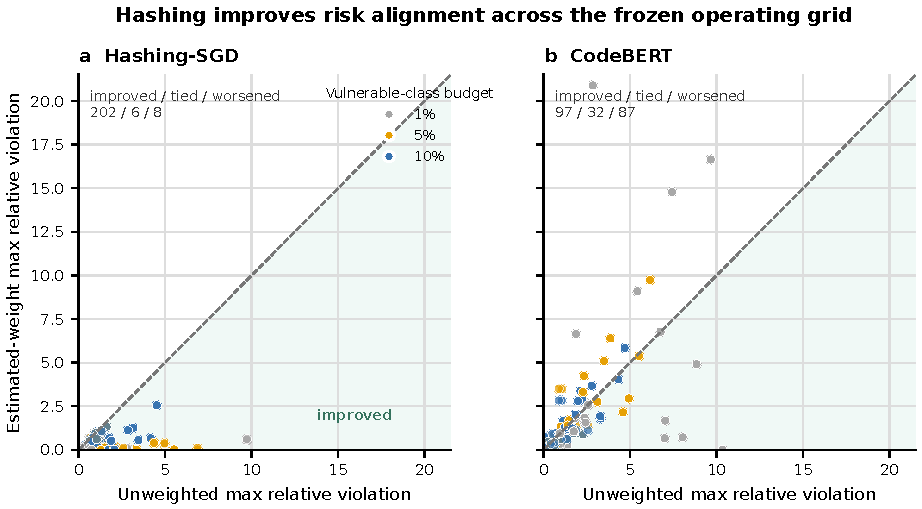
\includegraphics[width=0.94\textwidth]{fig4_risk_alignment.pdf}
  \caption{Directional risk alignment over 24 projects and nine frozen budget pairs. Each point compares estimated-weight sets with unweighted Mondrian sets; points below the diagonal improve maximum relative violation. Hashing-SGD improves in 202 of 216 cells and at the primary operating point in all 24 projects. Cell counts are descriptive because budget cells within a project are correlated.}
  \label{fig:alignment}
\end{figure*}

\subsection{The qualification firewall grants stable, detector-specific authority}

On the fixed registration half, hashing-SGD achieves severe-violation AUROC 0.7714, severe-project review rate 0.8000, and non-severe-project pass rate 0.7143. The resulting $Q=0.7571$ exceeds the registry threshold. The half held aside within the exploratory contract analysis strengthens the same result: AUROC, balanced triage accuracy, and $Q$ are all 0.9167. The registered contract makes seven projects eligible to request singleton automation; these comprise all six non-severe projects and one of six severe projects. The remaining five projects are review-only, and all five are severe. This 6/0/1/5 confirmation matrix shows that the registry decision and the runtime gate cooperate as intended: qualification grants the right to evaluate evidence, while the item-level contract still requires complete evidence and a valid singleton certificate.

The deterministic partition study shows that this result is not confined to the selected split. Hashing-SGD registers in 92.51\% of 10,000 registration halves, and both registration and confirmation halves exceed $Q=0.70$ in 84.94\% of splits. Its median $Q$ is 0.8286 in both halves, and the 10th percentile is 0.7222, still above the threshold. Thus, the qualification firewall is stable over a broad family of project allocations rather than being sustained by a few favorable projects.

The same mechanism provides a positive non-transfer result. CodeBERT's fixed registration score is $Q=0.1500$, so the registry withholds automation authority. Its confirmation score rises to 0.5909 but remains below threshold; all 12 confirmation projects are consequently review-only. Across 7,805 valid deterministic CodeBERT partitions, neither the registration half nor both halves qualify at $Q=0.70$. The firewall therefore prevents a successful hashing policy from being silently inherited by a detector whose threshold behavior does not support that authority.

\begin{figure*}[t]
  \centering
  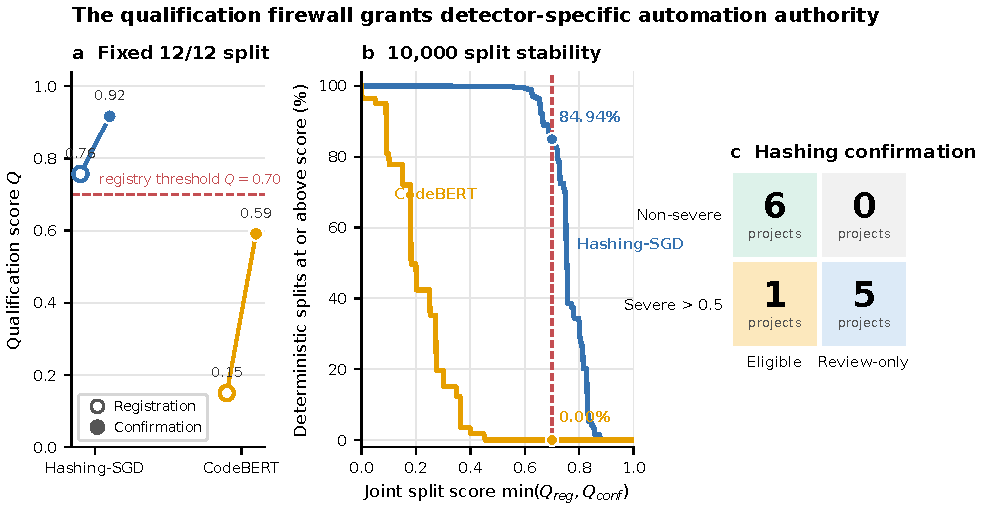
\includegraphics[width=0.96\textwidth]{fig2_gate_validity.pdf}
  \caption{Detector--shift qualification and confirmation. (a) The fixed registration half registers hashing-SGD above $Q=0.70$ and withholds CodeBERT; filled points show confirmation scores. (b) Survival curves report the proportion of deterministic 12/12 splits whose registration and confirmation scores both meet a candidate threshold; at $Q=0.70$, hashing-SGD retains 84.94\% and CodeBERT 0\%. (c) On the fixed hashing confirmation half, all six non-severe projects are eligible and five of six severe projects are review-only. Eligibility remains subject to item-level singleton and certificate checks.}
  \label{fig:gate}
\end{figure*}

Across the full 24-project cohort, the underlying hashing gate supplies the same direction: it routes 9 of 11 severe projects to review and passes 11 of 13 non-severe projects, with AUROC 0.8601 and AUPRC 0.8173. Table~\ref{tab:gate_ablation} isolates the evidence rules at clip 20. ESS alone passes every project, and infinity mass alone refuses four hashing projects without improving supported median risk. The full severe-risk rule is the only variant that reduces the supported hashing median from 0.483 to 0.122, which motivates its role inside $K_3$.

\begin{table*}[t]
\centering
\caption{Clip-20 evidence-rule ablation at $(\av,\as)=(0.10,0.20)$. For gate variants, medians are computed over support-pass projects; for the no-gate row, all 24 projects are included and support-pass is not applicable.}
\label{tab:gate_ablation}
\footnotesize
\begin{tabularx}{\textwidth}{@{}l*{6}{>{\centering\arraybackslash}X}@{}}
\toprule
& \multicolumn{3}{c|}{Hashing-SGD} & \multicolumn{3}{c}{CodeBERT} \\
Policy & Pass / 24 & Max rel. violation & Cov. & Pass / 24 & Max rel. violation & Cov. \\
\midrule
Weighted, no gate & n/a & 0.483 & 0.524 & n/a & 1.244 & 0.749 \\
ESS-only gate & 24 & 0.483 & 0.524 & 24 & 1.244 & 0.749 \\
Infinity-mass-only gate & 20 & 0.483 & 0.554 & 24 & 1.244 & 0.749 \\
Full frozen gate & 13 & 0.122 & 0.509 & 22 & 1.244 & 0.749 \\
\bottomrule
\end{tabularx}
\end{table*}

\subsection{Risk--coverage positioning makes review economics explicit}

At the primary operating point, the full controller supports 13/24 hashing projects. Within this qualified cohort, median singleton coverage is 50.9\% and median maximum relative violation is 0.122. The no-gate weighting effect carries a 15.9 percentage-point project-paired reduction in singleton coverage relative to unweighted Mondrian sets, making the automation price of improved alignment measurable rather than implicit. Two of the 13 supported projects attain both strict class budgets; this stricter endpoint is reported separately from the controller's severe-violation target.

Figure~\ref{fig:riskcoverage} positions these operating points against practical comparators. The qualified hashing controller combines a 0.122 supported median maximum relative violation with 50.9\% median singleton coverage, approximately twice the automation volume of PROM-derived APS/RAPS at their lowest-risk operating region. The unweighted-to-weighted arrow visualizes the substantial hashing risk reduction and its coverage cost. The CodeBERT panel functions as the paired transfer audit, keeping support qualification tied to the detector--shift pair.

\begin{figure*}[t]
  \centering
  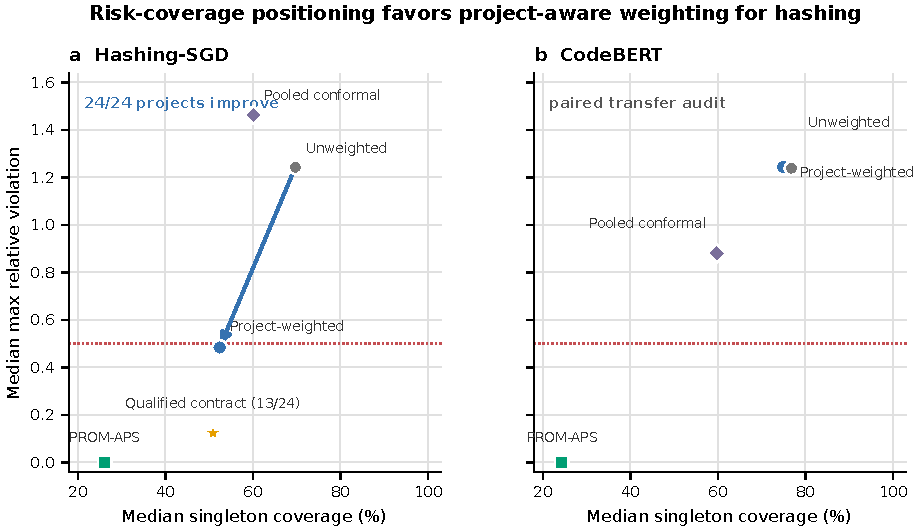
\includegraphics[width=0.94\textwidth]{fig3_primary_automation.pdf}
  \caption{Risk--coverage positioning at $(\av,\as)=(0.10,0.20)$. Points report project medians; the hashing star reports the qualified gate cohort. The arrow connects unweighted Mondrian sets to project-aware weighting. The CodeBERT panel retains only pre-contract operating points because its detector--shift identity is not registered.}
  \label{fig:riskcoverage}
\end{figure*}

\subsection{Sensitivity and resource observations}

The calibration-size sensitivity preserves the central detector contrast (Fig.~\ref{fig:calibration}). For hashing-SGD, weighted versus unweighted median maximum relative violation is 0.099 versus 1.271 at 25\% calibration, and 0.483 versus 1.242 at 100\%; weighted coverage rises from 35.5\% to 52.4\% while remaining below unweighted coverage of 69.4\% to 69.7\%. Full-gate pass rates rise from 0 at 25\% to 0.542 at 100\%, but the 25\% full-gate zero attainment is entirely review-only. CodeBERT has no consistent weighting advantage: its weighted maximum relative violation is 1.290, 1.296, 1.295, and 1.244 across the four fractions, versus 1.270, 1.224, 1.219, and 1.238 unweighted.

The near-duplicate audit generated 866,094 approximate-LSH candidates and exactly verified every candidate. It flagged 24,606 pairs at lexical-token Jaccard at least 0.90, affecting 15,026 of 79,355 target rows (18.94\%) and retaining 64,329 rows. Recomputing sealed decisions on the clean sensitivity cohort preserves the hashing direction: weighted maximum relative violation changes from 0.483 to 0.434 and coverage from 0.524 to 0.528, whereas CodeBERT changes from 1.244 to 1.799 and from 0.749 to 0.769. This is a sensitivity re-evaluation, not a refit.

\begin{figure*}[t]
  \centering
  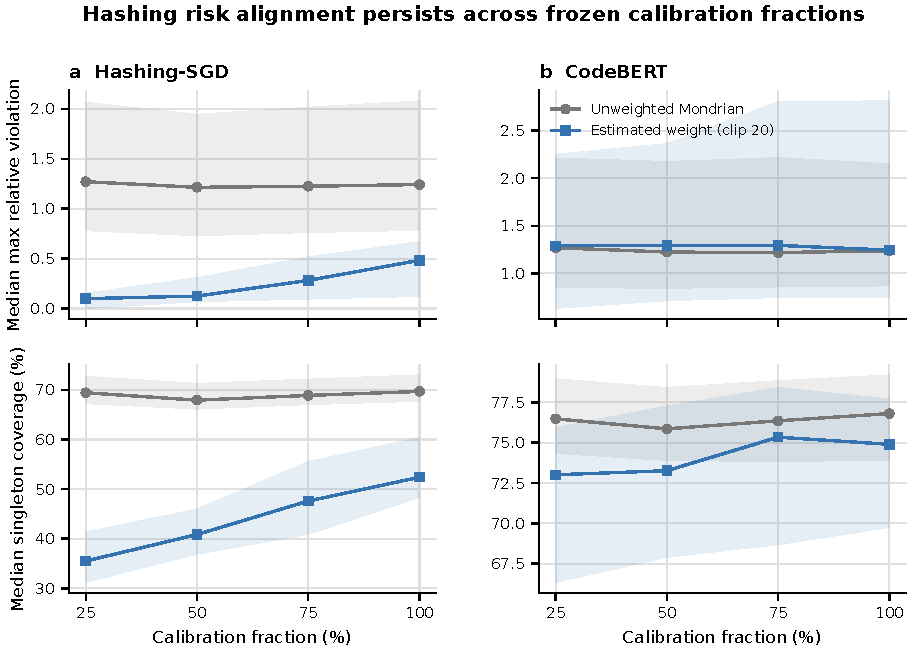
\includegraphics[width=0.94\textwidth]{fig5_calibration_sensitivity.pdf}
  \caption{Calibration-size sensitivity at the primary budget. Lines show project medians and ribbons show the interquartile range across 24 projects. Weighted hashing retains lower maximum relative violation at every fraction but lower singleton coverage; CodeBERT has no consistent risk-alignment advantage.}
  \label{fig:calibration}
\end{figure*}

The efficiency audit is observational. Hashing executes 120 independent head fits with a median 1.83 s fit duration, whereas CodeBERT executes 24 actual deterministic head fits with a median 1,584 s duration after 1,522 s of embedding extraction. CodeBERT runs in four concurrent parts; hashing is recorded as a sequential pipeline. Because hardware, batching, and parallelization differ, these numbers do not support a speedup, energy, or architecture-efficiency claim. They do support reporting the resource cost of the semantic track and the seed-reuse policy.

\section{Discussion}

\subsection{Answers to the research questions}

For RQ1, the executable contract supplies a mechanically checkable bridge from uncertainty evidence to action. The semantics guarantee automatic-action soundness relative to the serialized rules, fail-closed monotonicity under evidence loss, and detector-transfer non-interference. The implementation exercises these properties with unit tests that reject missing evidence, mismatched identities, altered entitlements, and auto-safe/auto-vulnerable action substitution. This is stronger than logging a confidence score after a decision: the decision carries the proof object required to verify its own authorization.

For RQ2, hashing-SGD passes registration at $Q=0.7571$, confirms at $Q=0.9167$, and qualifies on both halves in 84.94\% of deterministic partitions. The confirmation contract releases all six non-severe projects as eligible and routes five of six severe projects to review. CodeBERT is withheld at registration and therefore cannot inherit hashing authority. The registry consequently turns detector specificity from a narrative warning into an executable access-control decision.

For RQ3, project-aware weighting supplies the empirical foundation for that authority. All 24 hashing projects improve at the primary operating point, 202 of 216 frozen project--budget cells improve, and the paired median reduction is 0.8161. The direction persists at every frozen calibration fraction and after high-similarity target rows are removed. The 15.9 percentage-point singleton-coverage change makes the associated review demand explicit rather than hiding it inside aggregate accuracy.

\subsection{Knowledge contribution beyond abstention}

Selective prediction decides whether an individual score or set is sufficiently decisive. The proposed contract adds a distinct governance layer around that mechanism. First, authority is indexed by a detector--shift identity rather than attached globally to a model class. Second, evidence has an epistemic state: missing information is unknown, not silently false or imputed as pass. Third, an automatic action must carry a verifiable certificate that binds identity, budget, prediction set, rule evaluation, and evidence digest. Finally, a registry separates the evidence needed to qualify an authority from the evidence used to exercise it. These elements make \method a knowledge-based permission system for selective prediction, not merely another confidence threshold.

The CodeBERT result clarifies why this layer matters. CodeBERT has comparable base classification metrics and higher error-detection AUROC, yet its weighted risk alignment and threshold behavior do not support the hashing contract. A score-only workflow could still reuse the same gate and quietly automate. The qualification firewall instead converts this mismatch into a constructive outcome: unsupported transfer produces a review-only registry state with no change to the underlying detector.

\subsection{Operational implications}

A deployment can maintain a registry of detector--shift identities, require a new qualification whenever the detector, source domain, target domain, or policy version changes, and verify certificates before automatic labels enter downstream systems. Monitoring can then separate four quantities that answer different questions: registry qualification, runtime gate status, singleton coverage, and later label-revealed budget attainment. This separation makes review allocation auditable and supports policy revision without retraining the detector.

The public implementation exposes this workflow directly. It provides the contract module, deterministic registry analysis, decision tables, partition-stability scores, figure source data, and SHA-256 manifests. The result is an inspectable evidence chain from frozen detector outputs to a final action, which is the practical unit of value for knowledge-based security decision support.

\subsection{Scope and validity boundary}

The three formal properties are guarantees of the contract semantics, not guarantees that a detector is correct or that empirical class risks achieve finite-sample bounds. The learned density ratios are approximate and project shift may include conditional-label shift. We therefore keep empirical budget attainment separate from qualification, automation coverage, and certificate validity.

The qualification study is an explicitly exploratory extension over 24 public C/C++ projects. The fixed $Q=0.70$ threshold, 12/12 split, and 10,000 deterministic perturbations make sensitivity visible but do not create 10,000 independent samples. CodeBERT uses one deterministic head fit per project copied across seed addresses, and public vulnerability labels can contain omissions or noise. Extension to fine-tuned semantic detectors, other languages, private repositories, and human analyst productivity requires new identity-specific registration rather than inheritance from the present registry.

\subsection{Responsible-use boundary}

The study uses public source-code records and vulnerability labels for defensive classification. It does not generate exploits or access live systems, and it does not involve human participants. The method is evaluated as a decision-support layer for vulnerability triage, not as a security certification or an autonomous remediation system.

\section{Conclusion}

\method recasts cross-project vulnerability automation as a permission carried by evidence. Its detector--shift registry, three-valued knowledge rules, fail-closed semantics, and verifiable certificates make automatic actions inspectable and prevent authority from transferring silently across detectors. Hashing-SGD passes registration and confirms strongly, with both halves qualified in 84.94\% of deterministic partitions; the same firewall withholds CodeBERT authority. This governance result is supported by a frozen empirical foundation in which project-aware weighting improves hashing risk alignment on all 24 projects at the primary operating point and on 202 of 216 project--budget cells, with the direction preserved under sensitivity analyses. Proof-carrying knowledge contracts therefore provide a concrete architecture for turning selective predictions into auditable, detector-specific actions under software-project shift.

\section*{Funding}
This research did not receive any specific grant from funding agencies in the public, commercial, or not-for-profit sectors.

\section*{Declaration of competing interest}
The authors declare that they have no known competing financial interests or personal relationships that could have appeared to influence the work reported in this paper.

\section*{Data availability}
PrimeVul and DiverseVul are public defensive-use datasets released by their respective authors \cite{ding2025primevul,chen2023diversevul}. The public repository at \url{https://github.com/bianyanbo44-afk/vultriage-fcs} contains the frozen protocol, label-free source and target metadata, evaluation and analysis code, the executable knowledge-contract module, qualification and certificate tests, 10,000-partition stability scores, summary tables, figure source data, and validation manifests. It excludes raw source datasets, target-label vaults, private SQLite indexes, CodeBERT embeddings, feature caches, and per-function prediction or decision archives. The KBS submission source and PDF are supplied in the submission package; the GitHub link is the reproducibility artifact rather than a second authoritative copy of the manuscript. The extension-v2 configuration SHA-256 is \texttt{8AA39B09\allowbreak{}20D8CD2C\allowbreak{}FEFBF8C2\allowbreak{}8109754F\allowbreak{}1B2DFA60\allowbreak{}49E17565\allowbreak{}122C6968\allowbreak{}E199AAD2}; the contract-v1 configuration SHA-256 is \texttt{83779571\allowbreak{}9587D25D\allowbreak{}6EDB0BC6\allowbreak{}36D89AE5\allowbreak{}1385C364\allowbreak{}3677771B\allowbreak{}5BD1F186\allowbreak{}CAD1C946}.

\section*{Ethics statement}
The study uses public source-code records and vulnerability labels for defensive classification. It does not generate exploits, access live systems, or involve human participants; institutional ethics review is not applicable subject to institutional policy.

\section*{Declaration of generative AI and AI-assisted technologies in the manuscript preparation process}
During the preparation of this manuscript, the authors used OpenAI Codex, a generative-AI tool, to assist with research-question exploration, methodological planning, code drafting and debugging, analysis interpretation, and manuscript drafting. After using this tool, the authors reviewed and edited the content as needed and take full responsibility for the content of the published article. No generative AI was used to fabricate data, results, or figures.

\section*{CRediT authorship contribution statement}
Yanbo Bian: Conceptualization, Data curation, Formal analysis, Investigation, Methodology, Project administration, Software, Validation, Visualization, Writing--original draft, Writing--review and editing. Zhihai Wang: Conceptualization, Formal analysis, Methodology, Supervision, Validation, Writing--review and editing.

\bibliographystyle{elsarticle-num-names}
\bibliography{references}

\end{document}
